\documentclass[Eubank_pk_ethnic_sorting.tex]{subfiles}


\begin{document}

The key to determining whether the government-private test-score gap is caused by differences in quality or simply student sorting is understanding what motivates parents to pick one type of school over the other. This Section provides an overview of how households make these choices, and how those choices vary by village caste composition.

\subsection{Selection in Homogeneous Villages}\label{}

Parents in the LEAPS survey shown a marked tendency to invest preferentially in the children they view as having the most potential. As noted by the original LEAPS survey authors, ``through their choices of whether to enroll a child, through the choice of school ([government] or private) and finally through the amount they chose to spend, households pick ``winners'' and try to carry them through.'' \citep[p. 103]{Andrabi:2007we}

One manifestation of this is that conditional on sending their children to school, they are more likely to send their children to a private school if they perceive them as being more intelligent. This is illustrated in Table~\ref{hhselection} below, in which an indicator for whether an enrolled child attends a private school is regressed on parental perceptions of child intelligence and a number of demographic controls. The results show clearly that child intelligence are a strong predictor of whether a parent will send their child to a private school. Most notably, these results show this pattern holds even \emph{within individual households}. As shown in Column 2, which includes household fixed effects, many parents send the child they perceive to be more intelligent to private school and the child they perceive to be less intelligent to government schools.

\begin{table}[htbp]\centering
\def\sym#1{\ifmmode^{#1}\else\(^{#1}\)\fi}
\caption{School Choice and Child Intelligence\label{hhselection}}
\begin{tabular}{l*{2}{c}}
\hline\hline
                &\multicolumn{1}{c}{(1)}&\multicolumn{1}{c}{(2)}\\
                &\multicolumn{1}{c}{Village FE}&\multicolumn{1}{c}{HH FE}\\
\hline
Mom Reports Child Above Average Intelligence&    0.056***&    0.041*  \\
                &   (2.70)   &   (1.98)   \\
Mom Has Some Schooling&    0.080   &   -0.034   \\
                &   (1.43)   &  (-0.28)   \\
Dad Has Some Schooling&    0.082***&    0.085   \\
                &   (3.20)   &   (0.72)   \\
PCA Wealth Index&   -0.028   &        .   \\
                &  (-1.25)   &        .   \\
Age             &   -0.019***&   -0.017***\\
                &  (-3.45)   &  (-3.22)   \\
Age Squared     &  0.00025*  &  0.00017   \\
                &   (1.67)   &   (1.61)   \\
Female          &    0.035   &   0.0020   \\
                &   (1.59)   &   (0.07)   \\
\hline
Observations    &     3361   &     3361   \\
\hline\hline
\multicolumn{3}{l}{\footnotesize \textit{t} statistics in parentheses}\\
\multicolumn{3}{l}{\footnotesize * p<0.10, ** p<0.05, *** p<0.01}\\
\end{tabular}
\end{table}


The implications of this tendency for understanding the government-private test-score gap is clear: if parents are choosing to send their more academically-inclined children to private schools, and if parents have more information about student quality than researchers are able to measure in surveys and control for statistically, then standard analyses are likely to systematically overstate the quality of private school educations.

\subsection{Selection in Heterogeneous Villages}\label{}

While the tendency for parents to invest in ``winners'' rather than distribute resources uniformly is a consistent tendency in the LEAPS data, it is not the only factor that shapes school choice.  In more caste-heterogeneous villages, the \emph{social} composition of schools becomes increasing salient determinant. As shown below, as villages become more diverse, ``high status'' \emph{biraderis} become more likely to send their children to private schools, creating socially segregated schools where sorting is based on social factors in addition to perceived academic potential. 


To illustrate this, it is necessary to first grouping \emph{biraderis} into ``high'' and ``low'' social status groupings allows for a better understanding of segregation patterns. The crudeness of these categorizations is unfortunate, but necessary -- although \emph{biraderis} are associated with strict hierarchies within villages, there does not exist an explicit global hierarchy of \emph{biraderis} in Pakistan as in with the more familiar \emph{varna} caste designations India. As a result, these hierarchies may vary somewhat from village to village, and as noted previously, this variation may not perfectly follow economic position.

To estimate the social status of different \emph{biraderis}, Punjabi Pakistanis recruited on \emph{oDesk.com} were asked to classify \emph{biraderis} as having either ``high'' or ``low'' social status. Details of classifications can be found in Appendix~\ref{appendix_classification}.\footnote{This work has avoided the \cite{Jacoby:2011tc} methodology -- where castes are ranked on the basis of their land holding -- due to input from numerous sources that social standing and land holding are not equivalent, and in this exercise \emph{social}-status is of substantially more importance than \emph{socio-economic} status.}

Using these classifications, Table~\ref{highpooling} examines how school choice varies with student social standing and village composition. The results show that in villages with higher caste fractionalization, a larger share of private school students come from higher status \emph{biraderis} and a larger share of government school students come from low \emph{biraderis}. Private schools, in other words, become reservoirs of the social elite.

\begin{table}[htbp]\centering
\def\sym#1{\ifmmode^{#1}\else\(^{#1}\)\fi}
\caption{Student Social Status by School Type\label{highpooling}}
\begin{tabular}{l*{2}{c}}
\toprule
                &\multicolumn{1}{c}{(1)}&\multicolumn{1}{c}{(2)}\\
                &\multicolumn{1}{c}{Pct of Students High Status}&\multicolumn{1}{c}{Pct of Students High Status}\\
\midrule
Private School  &    -0.11** &    -0.13** \\
                &  (-2.30)   &  (-2.13)   \\
Biraderi Fractionalization&   -0.047*  &    -0.19***\\
                &  (-1.85)   & (-14.78)   \\
Fractionalization * Private&     0.18** &     0.21** \\
                &   (2.34)   &   (2.15)   \\
Median Village Expenditure&0.0000014   &            \\
                &   (0.87)   &            \\
Village: Pct Adults Literate&  0.00022   &            \\
                &   (1.22)   &            \\
Log Village Size&  0.00074   &            \\
                &   (0.16)   &            \\
Village: Pct High Status&     1.01***&            \\
                &  (62.12)   &            \\
Constant        &  -0.0039   &     1.00***\\
                &  (-0.10)   &  (83.16)   \\
District Fixed Effects&      Yes   &       No   \\
Village Fixed Effects&       No   &      Yes   \\
\midrule
Observations    &      782   &      782   \\
\bottomrule
\multicolumn{3}{l}{\footnotesize \textit{t} statistics in parentheses}\\
\multicolumn{3}{l}{\footnotesize * p<0.10, ** p<0.05, *** p<0.01}\\
\end{tabular}
\end{table}



Further evidence of social segregation in schooling is provided by Figure~\ref{schoolvvillageherf}, which plots the relationship between a village-level fragmentation index and intra-school fragmentation indices. If schools were unsegregated, then we would expected the herfindahl indices computed \emph{within} each school to track closely with herfindahl indices computed at the village level. Yet as shown in Figure~\ref{schoolvvillageherf}, this is far from the case. Almost all schools are below the 45 degree line that would indicate school and village diversity moving one for one, and many are well below.

\begin{figure}[H]
	\begin{center}
	\caption{School Versus Village Fragmentation}\label{schoolvvillageherf}
	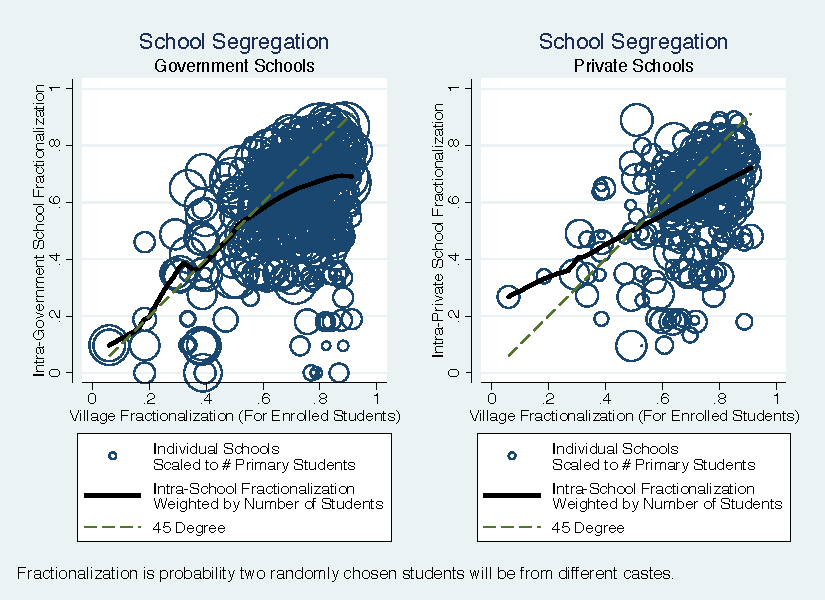
\includegraphics[scale=1.0]{../results/intra_versus_intervillage_frac_combined.pdf}
	\end{center}
\end{figure}

Demand for caste segregation is also manifest in the dramatically higher prices charged by segregated private schools. As shown in Table~\ref{fees} below, moving from a perfectly non-fractionalized village to a perfectly fractionalized village is associated with an average \input{../results/fee_avg_effect.tex} Rupees increase in annual school fees. Given that the median annual fee for all private schools in the LEAPS survey is \input{../results/fee_median_fee.tex} Rupees, this is a very significant amount.\footnote{Fees above the 95th percentile -- \input{../results/fee_windsor.tex} Rupees -- were adjusted down to \input{../results/fee_windsor.tex}  Rupees. Without this adjustment, the coefficient on village fractionalization is even larger.}

\begin{table}[htbp]\centering
\def\sym#1{\ifmmode^{#1}\else\(^{#1}\)\fi}
\caption{Annual Private School Fees\label{fees}}
\begin{tabular}{l*{3}{c}}
\toprule
                &\multicolumn{1}{c}{(1)}&\multicolumn{1}{c}{(2)}&\multicolumn{1}{c}{(3)}\\
                &\multicolumn{1}{c}{Weighted by School}&\multicolumn{1}{c}{Weighted by School}&\multicolumn{1}{c}{Weighted by Primary Students}\\
\midrule
Biraderi        &    504.7** &    527.9** &    608.6** \\
Fractionalization&   (2.33)   &   (2.50)   &   (2.37)   \\
Village: Median &            &     61.6   &     20.8   \\
Expenditures    &            &   (1.25)   &   (0.44)   \\
Expenditure Gini&            &    -49.9   &     45.5   \\
                &            &  (-0.24)   &   (0.20)   \\
District Fixed Effects &      Yes   &      Yes   &      Yes   \\
\midrule
Observations    &      287   &      287   &      285   \\
\bottomrule
\multicolumn{4}{l}{\footnotesize \textit{t} statistics in parentheses}\\
\multicolumn{4}{l}{\footnotesize * p<0.10, ** p<0.05, *** p<0.01}\\
\end{tabular}
\end{table}


Further, as shown in Table~\ref{privateshare}, none of these changes are driven by a change in the share of students in private schools. The percentage of students in private schools remains quite stable, even when controlling for numerous village characteristics.

\begin{table}[htbp]\centering
\def\sym#1{\ifmmode^{#1}\else\(^{#1}\)\fi}
\caption{Share of Enrolled Students in Private Schools \label{privateshare}}
\begin{tabular}{l*{2}{c}}
\toprule
                &\multicolumn{1}{c}{(1)}&\multicolumn{1}{c}{(2)}\\
                &\multicolumn{1}{c}{Share Students in Private School}&\multicolumn{1}{c}{Share Students in Private School}\\
\midrule
Biraderi Fractionalization&    0.077   &    0.085   \\
                &  (0.060)   &  (0.032)   \\
Median Village Expenditure&            & 0.000029** \\
                &            &(0.0000040)   \\
Village Land Gini&            &    0.022   \\
                &            &  (0.087)   \\
Village: Pct Adults Literate&            &   0.0019   \\
                &            & (0.0019)   \\
Log Num HHs     &            &    0.019   \\
                &            &  (0.022)   \\
District Fixed Effects&      Yes   &      Yes   \\
\midrule
Observations    &      112   &      112   \\
\bottomrule
\multicolumn{3}{l}{\footnotesize Standard errors in parentheses}\\
\multicolumn{3}{l}{\footnotesize * \(p<0.10\), ** \(p<0.05\), *** \(p<0.01\)}\\
\multicolumn{3}{l}{\footnotesize Results clustered at district level.}\\
\end{tabular}
\end{table}



\end{document}
